% Idee: Heno Ivanov
% Tekst: Heno Ivanov

\documentclass[a4paper,11pt]{article}
\usepackage[et]{../../eio}
\usepackage{tikz}

\begin{document}
\begin{ol}{\eio}{\ev 10.12.2023}{\yle}{}
\begin{yl}{4}{Sipelgas}{sipelgas}{1 sekund}{40 punkti}

Robotsipelgas liigub mööda kuubi servi. Sipelgas peatub alati kuubi tipus ja ootab käsku: käsu \verb|V| peale liigub ta järgmisse tippu mööda endast vasakul olevat serva, käsu \verb|P| peale mööda paremal olevat serva.

Kirjutada programm, mis saab sipelga poolt seni täidetud käskude jada ja leiab sipelga jaoks lühima võimaliku tee tagasi tippu, kust ta liikumist alustas.

\sis
Sisendi esimesel real on sipelga seni täidetud käskude arv $N$ ($0 \le N \le 1\,000$).
Teisel real on $N$ tähte \verb|V| ja \verb|P|: nende käskude loend.

\val 
Esimesele reale väljastada vähim käskude arv, millega saab sipelga suunata tagasi tippu, kust ta liikumist alustas.
Teisele reale väljastada selleks vajalik käskude loetelu (ühe sõnena, ilma tühikute või muude eraldajateta).
Kui minimaalse käskude arvuga teid lähtetippu on mitu, väljastada ükskõik milline neist.

\nde[0]{3cm}{3cm}

Alloleval joonisel näitavad punased noolekesed sipelga asukohta ja pea suunda ning sinised ja rohelised jooned vastavalt sisendis ja väljundis antud käskude järgi liikumisi.

\begin{center}
  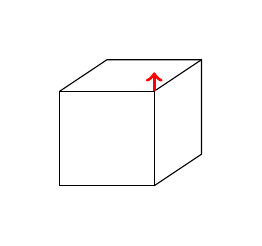
\begin{tikzpicture}[scale=0.4]
    \draw[white] (-1, -1) -- (5.5, -1) -- (5.5, 5) -- (-1, 5) -- (-1, -1);
    \draw (0, 0) -- (3, 0) -- (3, 3) -- (0, 3) -- (0, 0);
    \draw (3, 0) -- (4.5, 1) -- (4.5, 4) -- (3, 3);
    \draw (4.5, 4) -- (1.5, 4) -- (0, 3);
    \draw[->, red, very thick] (3, 3) -- (3, 3.6);
  \end{tikzpicture}
  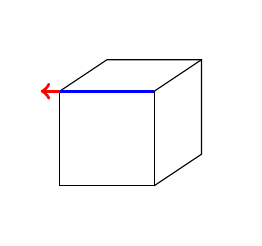
\begin{tikzpicture}[scale=0.4]
    \draw[white] (-1, -1) -- (5.5, -1) -- (5.5, 5) -- (-1, 5) -- (-1, -1);
    \draw (0, 0) -- (3, 0) -- (3, 3) -- (0, 3) -- (0, 0);
    \draw (3, 0) -- (4.5, 1) -- (4.5, 4) -- (3, 3);
    \draw (4.5, 4) -- (1.5, 4) -- (0, 3);
    \draw[blue, very thick] (3, 3) -- (0, 3);
    \draw[->, red, very thick] (0, 3) -- (-0.6, 3);
  \end{tikzpicture}
  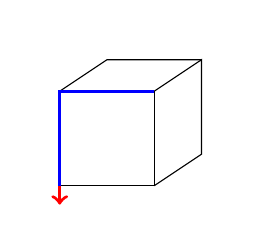
\begin{tikzpicture}[scale=0.4]
    \draw[white] (-1, -1) -- (5.5, -1) -- (5.5, 5) -- (-1, 5) -- (-1, -1);
    \draw (0, 0) -- (3, 0) -- (3, 3) -- (0, 3) -- (0, 0);
    \draw (3, 0) -- (4.5, 1) -- (4.5, 4) -- (3, 3);
    \draw (4.5, 4) -- (1.5, 4) -- (0, 3);
    \draw[blue, very thick] (3, 3) -- (0, 3) -- (0, 0);
    \draw[->, red, very thick] (0, 0) -- (0, -0.6);
  \end{tikzpicture}
  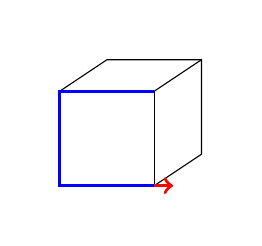
\begin{tikzpicture}[scale=0.4]
    \draw[white] (-1, -1) -- (5.5, -1) -- (5.5, 5) -- (-1, 5) -- (-1, -1);
    \draw (0, 0) -- (3, 0) -- (3, 3) -- (0, 3) -- (0, 0);
    \draw (3, 0) -- (4.5, 1) -- (4.5, 4) -- (3, 3);
    \draw (4.5, 4) -- (1.5, 4) -- (0, 3);
    \draw[blue, very thick] (3, 3) -- (0, 3) -- (0, 0) -- (3, 0);
    \draw[->, red, very thick] (3, 0) -- (3.6, 0);
  \end{tikzpicture}
  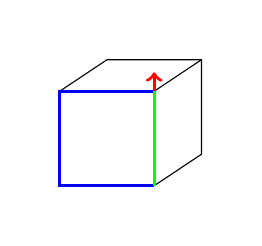
\begin{tikzpicture}[scale=0.4]
    \draw[white] (-1, -1) -- (5.5, -1) -- (5.5, 5) -- (-1, 5) -- (-1, -1);
    \draw (0, 0) -- (3, 0) -- (3, 3) -- (0, 3) -- (0, 0);
    \draw (3, 0) -- (4.5, 1) -- (4.5, 4) -- (3, 3);
    \draw (4.5, 4) -- (1.5, 4) -- (0, 3);
    \draw[blue, very thick] (3, 3) -- (0, 3) -- (0, 0) -- (3, 0);
    \draw[green, very thick] (3, 0) -- (3, 3);
    \draw[->, red, very thick] (3, 3) -- (3, 3.6);
  \end{tikzpicture}
\end{center}

\end{yl}
\end{ol}
\end{document}
